\chapter{Metodología de trabajo}

\label{sec:metodologia}

En este capítulo se describe la organización del proyecto, las herramientas metodológicas utilizadas y las herramientas usadas para la planificación de actividades, entre ellas destacan: la metodología basada en prototipos, el uso de SysML, los diagramas PERT y Gantt y la descomposición en objetos y tareas. A su vez, se realiza un análisis del proyecto utilizando estas herramientas y el anális de los riesgos.

\section{Metodología basada en prototipos}

La metodología basada en prototipos es un enfoque de desarrollo de proyectos que se utiliza para construir sistemas de software de manera iterativa e incremental. En el contexto de proyectos de software, la metodología basada en prototipos implica la creación de versiones preliminares o prototipos del sistema a lo largo del ciclo de desarrollo. Estos prototipos son versiones simplificadas del sistema final que permiten probar ideas, obtener retroalimentación y validar requisitos antes de la implementación completa.

Uno de los principales beneficios de esta metodología es su enfoque centrado en el usuario. Al desarrollar prototipos, se fomenta la participación activa de los usuarios y se recopila su retroalimentación temprana. Esto permite comprender mejor sus necesidades, expectativas y preferencias, lo que a su vez contribuye a la creación de un sistema final más alineado con sus requerimientos. Además, la metodología basada en prototipos ofrece la ventaja de la rapidez en el desarrollo. Al entregar prototipos funcionales en etapas tempranas del proyecto, se acelera el proceso de validación de conceptos y se reducen los tiempos de respuesta. Esto es especialmente beneficioso en proyectos con plazos ajustados o en entornos donde se requiere una rápida validación de ideas.

La flexibilidad y adaptabilidad son otros aspectos destacados de esta metodología. Los prototipos permiten realizar experimentos y explorar diferentes soluciones antes de comprometerse con una implementación final. Si se detectan problemas o limitaciones, es posible ajustar o cambiar el enfoque sin grandes implicaciones en el sistema completo. Esta flexibilidad facilita la evolución y mejora continua del sistema a medida que se obtiene más conocimiento y experiencia durante el desarrollo.

\subsection{Prototipos contemplados}

Se ha decidido seguir una metodología basada en prototipos debido a sus ventajas en este tipo de proyectos. A continuación se describirán cada uno de los tres prototipos creados que serán divididos en capítulos en el documento:

\begin{enumerate}
   \item \textbf{Prototipo de Exploración}: Se describe el desarrollo inicial del sistema por parte del hardware; la configuración de la Rasperry-Pi así como la conexión de los sensores junto con su implementación y las pruebas realizadas.
    \item \textbf{Prototipo Incremental}: Describe cómo puede utilizarse Erlang sobre la Raspberry-Pi 3 así como diferentes métodos de instalación de este lenguaje sobre la misma, por último, se presentan pruebas realizadas con la placa R-Pi utilizando Erlang.
    \item \textbf{Prototipo Funcional}: Se relata como se ha creado el servidor y cada una de sus partes así como el código que lo implementa, a mayores se describen las pruebas de carga realizadas sobre el mismo para evaluar su rendimiento.

    
\end{enumerate}
\section{Lenguaje de Modelado - SysML}

Para el modelado del análisis y el diseño de los prototipos se utilizará SYSML (\emph{Systems Modeling Language} -- Lenguaje de Modelado de Sistemas, en español). SysML Es un lenguaje de modelado con una componente gráfica importante, ampliamente utilizado en el entorno de la Ingeniería de Sistemas para describir, diseñar y analizar sistemas complejos, se usa especialmente en el diseño de sistemas en ingeniería mecánica, eléctrica, electrónica y de software.

Se basa en el estándar UML (Lenguaje de Modelado Unificado) y utiliza una notación gráfica para describir diferentes aspectos de un sistema, como su estructura, comportamiento, requisitos y análisis. Se compone de nueve tipos de diagramas, cada uno de los cuales se utiliza para describir diferentes aspectos del sistema y son los siguientes:

\begin{enumerate}

\item Diagrama de bloques: Se usa para representar la estructura y las relaciones funcionales entre los componentes de un sistema.
\item Diagrama de bloques internos: Utilizado para para representar la estructura interna de un bloque.
\item Diagrama de flujo de datos: Se utiliza para representar como fluyen los datos a través del sistema.
\item Diagrama de actividades: Se utiliza para modelar el comportamiento del sistema como una secuencia de acciones o actividades.
\item Diagrama de casos de uso: Se utiliza para representar las interacciones entre el sistema y sus usuarios o actores.
\item Diagrama de secuencia: Se utiliza para representar como los diferentes componentes de un sistema interactúan entre sí durante un proceso o escenario específico.
\item Diagrama de estado: Utilizado para representar los diferentes estados que puede tener un objeto en el sistema y como cambia entre ellos.
\item Diagrama de requisitos: Se utiliza para representar los requisitos del sistema y como se relacionan entre sí.
\item Diagrama de asignación de requisitos: Utilizado para representar cómo se asignan los requisitos a los componentes del sistema.
\end{enumerate}
SysML es una herramienta muy útil para el diseño y análisis de sistemas complejos, ya que permite a los ingenieros modelar y comprender el sistema en su totalidad, identificar posibles problemas y evaluar diferentes alternativas de diseño antes de la implementación.

En el diagrama de la Figura~\ref{fig:SYSML} pueden observarse los tipos de diagramas existentes y su respectiva distribución.

\begin{figure}[ht]
\centering
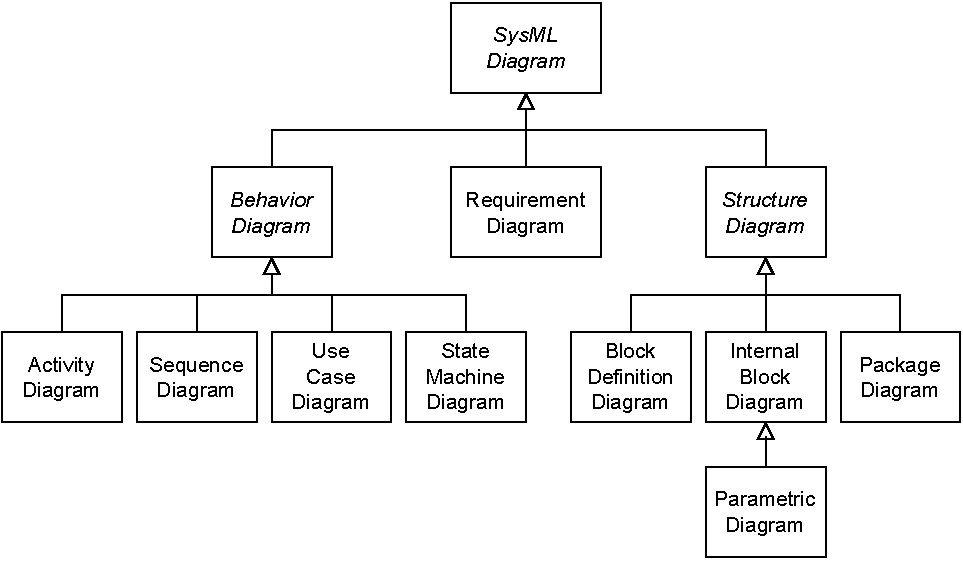
\includegraphics{images/SysMLDiagram.pdf}
\caption[Tipos de diagramas SysML]{Digrama que contiene los tipos de diagramas existentes en SysML.}%
\label{fig:SYSML}
\end{figure}

\section{Planificación del proyecto}

En la siguiente sección se discutirá la planificación del proyecto que se realiza en el Trabajo de Fin de Grado valorando los riesgos y utilizando diagramas de diferentes tipos para representar lo expuesto.

\subsection{Riesgos}%
\label{sec:riesgos}

Dentro de esta sección se analizarán  todos aquellos riegos por los que el proyecto puede verse afectado. Estos riesgos podrían suponer tanto un retraso en la fecha de entrega del proyecto, de alguna de las fases del proyecto hasta llegar a causar un aumento de los costes o incluso la no finalización del mismo. Estos riesgos serán analizados teniendo en cuenta la probabilidad que sucedan, el posible impacto que tengan en el proyecto y las posibles soluciones que puedan existir.

Los riesgos encontrados en este proyecto se pueden ver enumerados en el la Tabla~\ref{tabla:riesgos}. 

\begin{table}[htbp]
\begin{center}
\begin{tabular}{|l|l|}
\hline
\textbf{Código} & \textbf{Descripción} \\
\hline \hline
R-01 & Ausencia puntual del desarrollador. \\ \hline
R-02 & Fallo del equipo de trabajo. \\ \hline
R-03 & Fallo en componentes hardware utilizados. \\ \hline
R-04 & Cierre del laboratorio o centro de trabajo. \\ \hline
R-05 & Pérdida del trabajo realizado. \\ \hline
R-06 & Falta de conocimientos del desarrollador. \\ \hline
R-07 & Falta o retraso de material para el proyecto. \\ \hline
R-08 & Mala planificación del proyecto. \\ \hline
R-09 & Cambios en los requisitos del proyecto. \\ \hline
R-10 & Problemas de interoperabilidad. \\ \hline
\end{tabular}
\caption[Riesgos del sistema]{Enumeración de los riesgos junto con su código.}
\label{tabla:riesgos}
\end{center}
\end{table}

A continuación, se detallará para cada uno de los riesgos encontrados (identificados por su código), el impacto que pueden tener sobre el proyecto, la posibilidad de que ocurran y como podrían solucionarse o moderarse se mostrará en las tablas referenciadas.

\begin{itemize}
    \item \textbf{R-01}: La ausencia temporal del desarrollador debida a cualquier causa (enfermedad o asuntos personales) hace que el riesgo de aumento de duración del proyecto sea directamente proporcional al tiempo que dure la ausencia del mismo (~\ref{tabla:r-01}).
    \item \textbf{R-02}: El fallo del equipo de trabajo, en este caso el PC personal del desarrollador, puede llevar a demoras en el proyecto e incluso derivar en el riesgo R-05 (Pérdida del trabajo realizado) en caso de no haber almacenado información en la nube (~\ref{tabla:r-02}).
    \item \textbf{R-03}: El fallo de componentes hardware es común cuando se realizan trabajos de electricidad y se realizan pruebas sobre los componentes.(\ref{tabla:r-03}).
    \item \textbf{R-04}: El cierre del centro de trabajo, tras los eventos ocurridos durante el COVID-19, resulta más probable que nunca, este riesgo recoge la posibilidad de que el centro de trabajo o investigación tenga que cerrar sus puertas por un tiempo indefinido debido a causas internas o externas al mismo.(\ref{tabla:r-04}).
    \item \textbf{R-05}: Siempre existe la posibilidad de que algún equipo falle y se pierda la información almacenada hasta el momento. Este riesgo haría que el tiempo de entrega del proyecto se retrasara notablemente debido a que recuperar la información o volver a realizar el trabajo requiere mucho tiempo (~\ref{tabla:r-05}).
    \item \textbf{R-06}: La falta de formación del desarrollador para abordar el proyecto haría que este se viese comprometido. La probabilidad de que esto ocurra suele ser baja, pues para que el desarrollador sea seleccionado para el proyecto tiene que demostrar que conoce las herramientas con las que va a trabajar y que tiene conocimientos más que suficientes para llevarlo a cabo (~\ref{tabla:r-06}).
    \item \textbf{R-07}: La falta de material para el proyecto es habitual si no se realiza una planificación adecuada del trabajo, puede influir en el avance del mismo o llevar a cambios de plan. Siempre es recomendable tener suficiente stock para afrontar cualquier proyecto (~\ref{tabla:r-07}).
    \item \textbf{R-08}: La mala planificación del proyecto puede hacer que este se retrase o incluso que no pueda llevarse a cabo, es importante contar con improvistos y realizar una planificación detallada antes de comenzar el trabajo (~\ref{tabla:r-08}).
    \item \textbf{R-09}: Los cambios en los requisitos del proyecto son un riesgo frecuente debido a la modificación de los objetivos o la aparición de imprevistos.(~\ref{tabla:r-09}).
    \item \textbf{R-10}: Los problemas de interoperabilidad son un riesgo común en la realización de este tipo de proyectos debido al uso de diferentes lenguajes, sistemas operativos y componentes, este riego puede crear impedimentos en el flujo del plan de trabajo.(~\ref{tabla:r-10}).
\end{itemize}
    
\begin{table}[htbp]
\begin{center}
\begin{tabular}{|l|p{12cm}|}
\hline
\textbf{R-01} & Ausencia puntual de desarrollador. \\ \hline
\textbf{Impacto} & Bajo. \\ \hline
\textbf{Probabilidad} & Baja. \\ \hline
\textbf{Moderación} & Dar al desarrollador el tiempo que necesite hasta su vuelta. \\ \hline
\textbf{Medidas} & Asignar un desarrollador de respaldo o establecer un plan de contingencia para cubrir las ausencias. También se puede realizar una adecuada documentación y transferencia de conocimientos para que otros miembros del equipo puedan asumir el rol temporalmente.\\ \hline
\end{tabular}
\caption[Riesgo R-01]{Impacto, probabilidad, moderación y medidas del Riesgo R-01}
\label{tabla:r-01}
\end{center}
\end{table}
 
\begin{table}[htbp]
\begin{center}
\begin{tabular}{|l|p{12cm}|}
\hline
\textbf{R-02} & Fallo del equipo de trabajo. \\ \hline
\textbf{Impacto} & Bajo. \\ \hline
\textbf{Probabilidad} & Baja. \\ \hline
\textbf{Moderación} & Tener siempre repuesto de todos los equipos con los que se trabajen y almacenar la información en la nube o realizar copias de seguridad.\\ \hline
\textbf{Solución} & Realizar un mantenimiento preventivo regular de los equipos, incluyendo actualizaciones de software y hardware. Establecer políticas de respaldo y recuperación de datos. Contar con un plan de contingencia que incluya disponibilidad de equipos de respaldo en caso de fallo. Además, es importante contar con un soporte técnico confiable para resolver los problemas de manera rápida y eficiente.\\ \hline
\end{tabular}
\caption[Riesgo R-02]{Impacto, probabilidad, moderación y medidas del Riesgo R-02}
\label{tabla:r-02}
\end{center}
\end{table}  

\begin{table}[htbp]
\begin{center}
\begin{tabular}{|l|p{12cm}|}
\hline
\textbf{R-03} & Fallo en componentes hardware utilizados. \\ \hline
\textbf{Impacto} & Variable (depende de la criticidad del componente). \\ \hline
\textbf{Probabilidad} & Media. \\ \hline
\textbf{Moderación} & Comprobar los componentes antes de utilizarlos y revisar frecuentemente conexiones e implementaciones para evitar cortos o picos de potencia. \\ \hline
\textbf{Solución} & Realizar una adecuada evaluación y selección de los componentes hardware. Mantener un control de calidad en la adquisición y uso de los componentes. En caso de fallo, se debe buscar una solución de reemplazo o reparación lo más rápido posible, considerando la disponibilidad y compatibilidad de los componentes.\\ \hline
\end{tabular}
\caption[Riesgo R-03]{Impacto, probabilidad, moderación y medidas del Riesgo R-03}
\label{tabla:r-03}
\end{center}
\end{table} 

\begin{table}[htbp]
\begin{center}
\begin{tabular}{|l|p{12cm}|}
\hline
\textbf{R-04} & Cierre del laboratorio o centro de trabajo. \\ \hline
\textbf{Impacto} & Alto. \\ \hline
\textbf{Probabilidad} & Baja. \\ \hline
\textbf{Moderación} & No existe forma de moderación hasta que se resuelvan los asuntos que mantienen el centro cerrado. \\ \hline
\textbf{Solución} & Contar con un plan de contingencia que permita trasladar el trabajo a otro lugar en caso de cierre temporal o permanente del laboratorio o centro de trabajo. Esto podría incluir la utilización de instalaciones alternativas, el trabajo remoto o la reubicación de los recursos y equipos necesarios.\\ \hline
\end{tabular}
\caption[Riesgo R-04]{Impacto, probabilidad, moderación y medidas del Riesgo R-04}
\label{tabla:r-04}
\end{center}
\end{table} 

\begin{table}[htbp]
\begin{center}
\begin{tabular}{|l|p{12cm}|}
\hline
\textbf{R-05} & Pérdida del trabajo realizado. \\ \hline
\textbf{Impacto} & Alto. \\ \hline
\textbf{Probabilidad} & Baja. \\ \hline
\textbf{Moderación} & Realizar copias de seguridad periódicas del trabajo realizado, preferiblemente en múltiples ubicaciones o medios de almacenamiento. Utilizar sistemas de control de versiones y almacenamiento en la nube para evitar la pérdida de datos. Implementar prácticas de gestión de cambios adecuadas y realizar pruebas de recuperación de datos de manera regular. \\ \hline
\textbf{Solución} & Recuperar la información en caso de poder o rehacer todo desde la última versión recuperable.\\ \hline
\end{tabular}
\caption[Riesgo R-05]{Impacto, probabilidad, moderación y medidas del Riesgo R-05}
\label{tabla:r-05}
\end{center}
\end{table} 
 
\begin{table}[htbp]
\begin{center}
\begin{tabular}{|l|p{12cm}|}
\hline
\textbf{R-06} & Falta de conocimientos del desarrollador. \\ \hline
\textbf{Impacto} & Alto. \\ \hline
\textbf{Probabilidad} & Baja. \\ \hline
\textbf{Moderación} & Tener siempre bien formado a todo el equipo de desarrollo. \\ \hline
\textbf{Solución} & Proporcionar formación y capacitación adecuada al desarrollador para cubrir las lagunas de conocimiento identificadas. Asignar mentores o expertos en el área para brindar orientación y apoyo. En casos extremos, considerar la contratación de un desarrollador con las habilidades requeridas.\\ \hline
\end{tabular}
\caption[Riesgo R-06]{Impacto, probabilidad, moderación y medidas del Riesgo R-06}
\label{tabla:r-06}
\end{center}
\end{table}

\begin{table}[htbp]
\begin{center}
\begin{tabular}{|l|p{12cm}|}
\hline
\textbf{R-07} & Falta o retraso de material para el proyecto. \\ \hline
\textbf{Impacto} & Bajo. \\ \hline
\textbf{Probabilidad} & Media. \\ \hline
\textbf{Moderación} & Tener siempre suficiente stock de material. \\ \hline
\textbf{Solución} & Realizar una planificación adecuada del proyecto que incluya la identificación y adquisición temprana de los materiales necesarios. Establecer relaciones con proveedores confiables y asegurar acuerdos claros en términos de entrega y disponibilidad de los materiales. En caso de retraso, se puede buscar alternativas o reprogramar las actividades afectadas.\\ \hline
\end{tabular}
\caption[Riesgo R-07]{Impacto, probabilidad, moderación y medidas del Riesgo R-07}
\label{tabla:r-07}
\end{center}
\end{table}

\begin{table}[htbp]
\begin{center}
\begin{tabular}{|l|p{12cm}|}
\hline
\textbf{R-08} & Mala planificación del proyecto. \\ \hline
\textbf{Impacto} & Alto \\ \hline
\textbf{Probabilidad} & Baja \\ \hline
\textbf{Moderación} & Disponer de un plan realista y detallado y contar con improvistos. \\ \hline
\textbf{Solución} & Realizar una planificación detallada y realista del proyecto, considerando todos los aspectos relevantes, como recursos, plazos, objetivos y riesgos. Realizar un seguimiento continuo del progreso y ajustar la planificación según sea necesario. Contar con un equipo de gestión de proyectos competente y utilizar herramientas y metodologías adecuadas para la planificación y el control del proyecto.\\ \hline
\end{tabular}
\caption[Riesgo R-08]{Impacto, probabilidad, moderación y medidas del Riesgo R-08}
\label{tabla:r-08}
\end{center}
\end{table}

\begin{table}[htbp]
\begin{center}
\begin{tabular}{|l|p{12cm}|}
\hline
\textbf{R-09} & Cambios en los requisitos del proyecto. \\ \hline
\textbf{Impacto} & Variable (Depende de la magnitud de los cambios y su impacto en el proyecto). \\ \hline
\textbf{Probabilidad} & Alta. \\ \hline
\textbf{Moderación} & Contar con la posibilidad de modificación de los requisitos.\\ \hline
\textbf{Solución} & Establecer un proceso formal de gestión de cambios que permita evaluar, documentar y aprobar los cambios en los requisitos. Mantener una comunicación constante con los stakeholders para comprender y anticipar posibles cambios. Realizar revisiones regulares de los requisitos y adaptar el plan del proyecto en consecuencia.\\ \hline
\end{tabular}
\caption[Riesgo R-09]{Impacto, probabilidad, moderación y medidas del Riesgo R-09}
\label{tabla:r-09}
\end{center}
\end{table}

\begin{table}[htbp]
\begin{center}
\begin{tabular}{|l|p{12cm}|}
\hline
\textbf{R-10} & Problemas de interoperabilidad. \\ \hline
\textbf{Impacto} & Variable (Depende del grado de dependencia del proyecto de la interoperabilidad). \\ \hline
\textbf{Probabilidad} & Alta \\ \hline
\textbf{Moderación} & Investigar bien los componentes y sistemas antes de utilizarlos.\\ \hline
\textbf{Solución} & Realizar pruebas exhaustivas de interoperabilidad entre los componentes de hardware y software utilizados en el proyecto. Establecer estándares y protocolos de comunicación claros y asegurarse de que todos los elementos del proyecto cumplan con ellos. En caso de identificar problemas de interoperabilidad, trabajar en colaboración con los proveedores y fabricantes para resolverlos o buscar alternativas que sean compatibles.\\ \hline
\end{tabular}
\caption[Riesgo R-10]{Impacto, probabilidad, moderación y medidas del Riesgo R-10}
\label{tabla:r-10}
\end{center}
\end{table}

\clearpage
En la Figura~\ref{fig:matrizRiesgos} se muestra la matriz de probabilidad-impacto de los riesgos que se han identificado mediante su ID, se observa una linea de tolerancia y una distribución por colores para ver de manera visual qué riesgos han de tenerse más en cuenta para tomar medidas antes de que ocurran o disponer de soluciones en caso de que no sea posible evitarlos.

\begin{figure}[h]
\centering
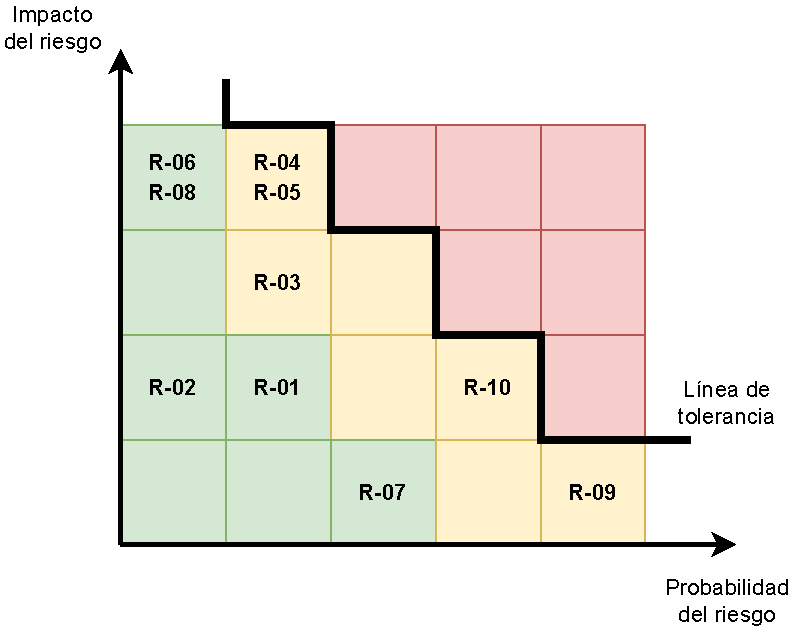
\includegraphics{images/matrizImpacto.pdf}
\caption[Matriz de impacto de riesgos]{Matriz de probabilidad.impacto de riesgos con los IDs de riesgos.}%
\label{fig:matrizRiesgos}
\end{figure}

\newpage

\subsection{Product Breakdown Structure}

La Product Breakdown Structure (PBS) es una herramienta utilizada en la gestión de proyectos para descomponer un producto o proyecto en componentes más pequeños y manejables. Se representa en forma de una estructura jerárquica que muestra la descomposición de alto nivel del producto en sus componentes más detallados.

La PBS se utiliza para definir y organizar las entregas y los elementos del producto. Cada nivel de la estructura representa un nivel de detalle mayor, desglosando el producto en sus partes constituyentes. Los elementos de la PBS se organizan de forma jerárquica, donde los niveles superiores representan las categorías principales y los niveles inferiores representan los elementos más específicos o detallados. Esta herramienta ayuda a visualizar y comprender la estructura del producto, identificar las partes y componentes clave, y establecer una base sólida para la planificación y el control del proyecto. Permite una gestión más efectiva de los recursos, la asignación de responsabilidades y la programación de las actividades necesarias para desarrollar y entregar el producto.

En la Figura~\ref{fig:PBS} pueden observarse el esquema PBS creado para este proyecto, el cual descompone en productos los prototipos necesarios para la realización del mismo así como cada uno de sus componentes.

\begin{figure}[ht]
\centering
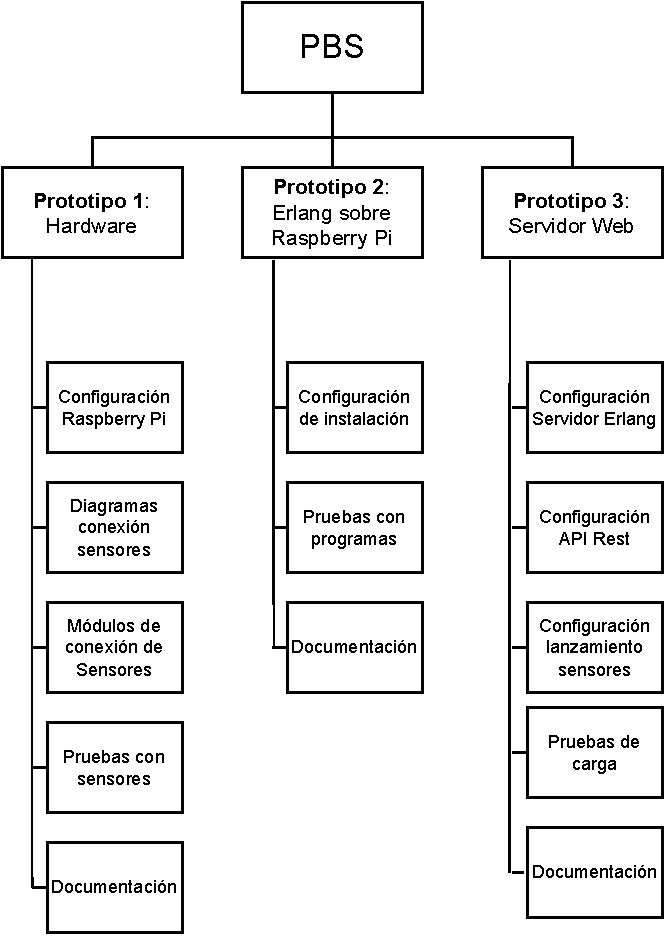
\includegraphics[scale=1.2]{images/PBS.pdf}
\caption[PBS del proyecto]{Esquema de la Product Breakdown Structure (PBS) realizada para la descomposición en objetos del proyecto.}%
\label{fig:PBS}
\end{figure}

\subsection{Work Breakdown Structure}

La Work Breakdown Structure (WBS) es una herramienta clave en la gestión de proyectos que descompone un proyecto en componentes más pequeños y manejables, conocidos como actividades o tareas. La WBS organiza y estructura el alcance del proyecto de manera jerárquica, dividiéndolo en niveles de detalle que representan las diferentes etapas, fases o entregables del proyecto.

La WBS se presenta como un árbol o estructura en la que cada nivel inferior representa una descomposición más detallada de las actividades del proyecto. En la parte superior se encuentra el nivel más general, que representa el alcance principal o los entregables principales del proyecto. A medida que se desciende en la estructura, se especifican las actividades más específicas y se definen las relaciones de dependencia entre ellas. Esta herramienta permite una comprensión clara y organizada del trabajo que debe realizarse en el proyecto. Al descomponer el proyecto en actividades más pequeñas y manejables, se facilita la asignación de responsabilidades a los miembros del equipo y se establece una base para la programación, estimación de recursos y presupuesto.

Los beneficios de utilizar WBS en la gestión de proyectos son diversos. Permite una mejor gestión del alcance, ya que todas las actividades necesarias para completar el proyecto están identificadas y organizadas. Además, ayuda a establecer una secuencia lógica de las actividades y a identificar las dependencias entre ellas. También facilita la comunicación y el seguimiento del progreso del proyecto, ya que proporciona una estructura clara y comprensible para todos los interesados. Permite una asignación eficiente de recursos y tiempo, al permitir la identificación de las actividades críticas y la planificación de los hitos clave del proyecto.

En la Figura~\ref{fig:WBS} pueden observarse el esquema WBS creado para este proyecto, el cual descompone en tareas la creación de los prototipos necesarios para la realización del mismo así como cada una de sus subtareas.

\begin{figure}[ht]
\centering
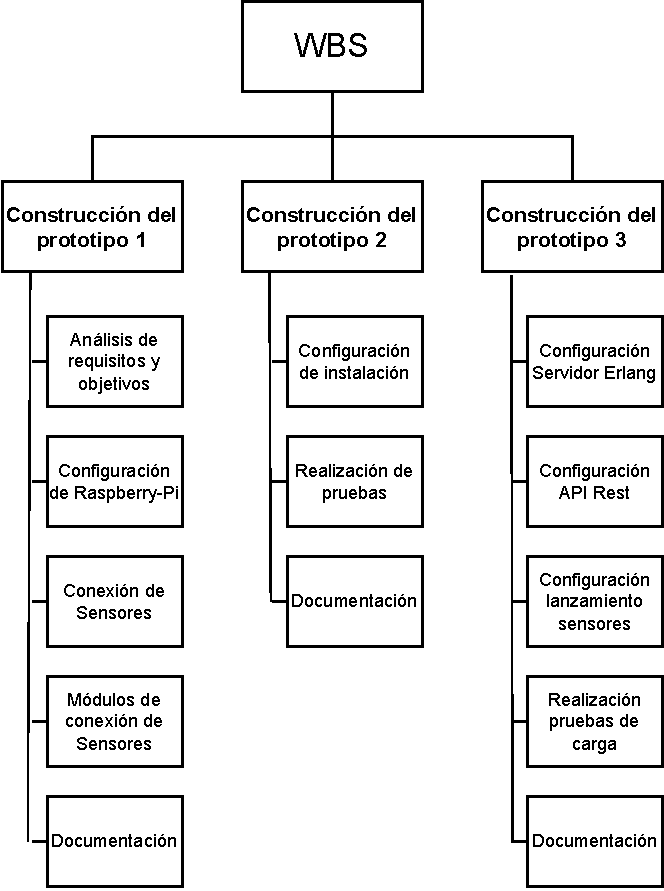
\includegraphics[scale=1.2]{images/WBS.pdf}
\caption[WBS del proyecto]{Esquema de la Work Breakdown Structure (WBS) realizada para la descomposición en tareas del proyecto.}%
\label{fig:WBS}
\end{figure}

\cleardoublepage

\subsection{Red de actividades del proyecto}

En este proyecto se ha plasmado la red de actividades como un diagrama PERT.

Los diagramas PERT (Program Evaluation and Review Technique) son herramientas utilizadas en la gestión de proyectos para visualizar y planificar las actividades y la secuencia de eventos en un proyecto. Estos diagramas se basan en la representación gráfica de las actividades del proyecto, así como en las relaciones de dependencia entre ellas. En un diagrama PERT, las actividades se representan mediante nodos o cajas, y las flechas indican las dependencias y el flujo de trabajo entre las actividades. Cada actividad se representa con su nombre y su duración estimada. Además, se pueden incluir hitos o eventos importantes en el proyecto.

Este tipo de diagramas ayuda a identificar las actividades críticas, es decir, aquellas actividades que tienen un impacto directo en la duración total del proyecto. Estas actividades críticas deben completarse dentro de los plazos establecidos para asegurar que el proyecto se complete a tiempo. Los beneficios de utilizar estos diagramas incluyen una mejor planificación y programación de proyectos, una mayor comprensión de las dependencias entre actividades, la identificación de las actividades críticas, la evaluación de riesgos y la capacidad de ajustar la programación en caso de cambios o retrasos.

En la Figura~\ref{fig:pert} puede observarse el diagrama PERT creado para la representación de las actividades a realizar en el proyecto, en él pueden distinguirse aquellas que tienen dependencias y su flujo de trabajo.

A través de este diagrama puede obtenerse la ruta crítica que se refiere a la secuencia de actividades que determina la duración más larga posible de un proyecto. Es la cadena de tareas que no pueden retrasarse sin retrasar la finalización del proyecto en su conjunto, es por ello que a estas actividades se les debe dar un plazo algo superior para evitar retrasos importantes en la duración del proyecto. La ruta obtenida es la siguiente:\\

\dirtree{%
.1 Configuración inicial Raspberry-Pi.
.2 Elección y conexión de sensores con Raspberry-Pi.
.3 Creación módulos de sensores.
.4 Creación Servidor Erlang.
.5 Configuración API REST.
.6 Lanzamiento sensores desde servidor.
.7 Pruebas finales.
.8 Documentación prototipo final.
}

\begin{figure}[p]
\centering
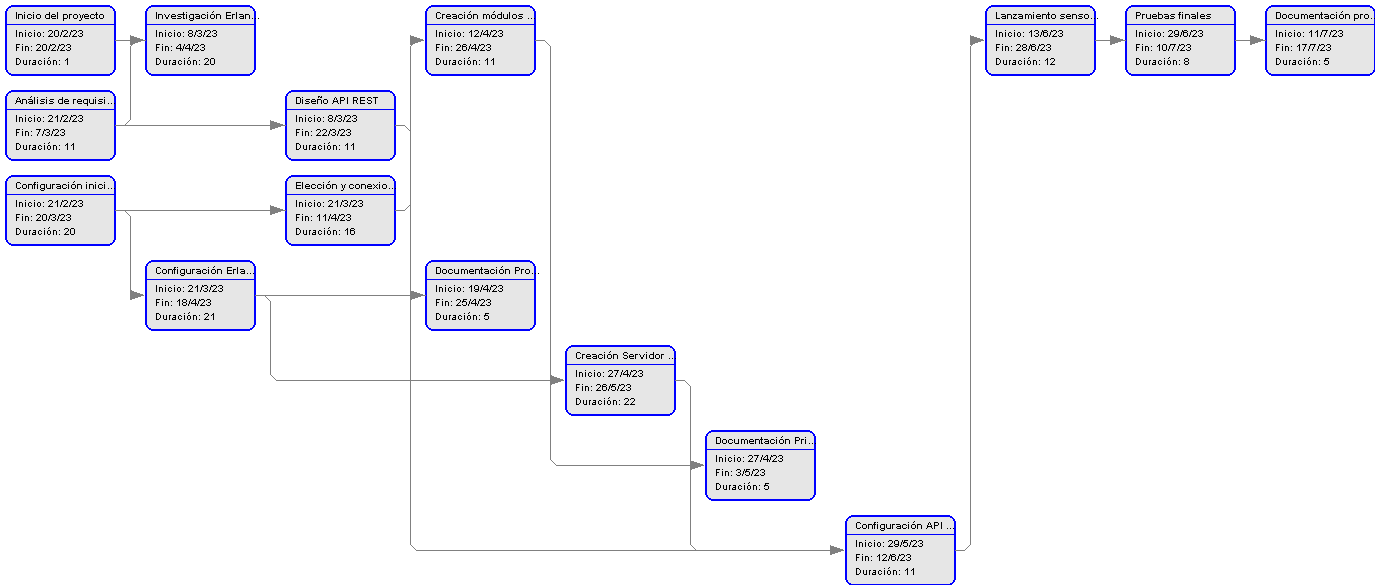
\includegraphics[scale=0.5,angle=90]{images/Pert.png}
\caption[Diagrama PERT]{Diagrama PERT de descomposición de actividades del proyecto}%
\label{fig:pert}
\end{figure}

\clearpage
\subsection{Diagrama de Gantt}

Un diagrama de Gantt es una herramienta de gestión de proyectos que muestra la planificación y programación de las actividades a lo largo del tiempo. Consiste en una representación gráfica en forma de barras horizontales que muestran la duración de cada actividad y su ubicación en el calendario. En un diagrama de Gantt, el eje horizontal representa el tiempo, generalmente en unidades de días, semanas o meses. Cada actividad se representa como una barra en el diagrama, donde la longitud de la barra indica la duración de la actividad. Las barras se colocan en el tiempo correspondiente en el eje horizontal y se pueden superponer si hay actividades que se solapan en el tiempo. Además de mostrar la duración de las actividades, el diagrama de Gantt también puede mostrar otras información relevante, como las dependencias entre actividades, los hitos importantes del proyecto y las fechas límite. Las dependencias se representan mediante flechas que indican la secuencia en la que las actividades deben llevarse a cabo.

Uno de los beneficios de estos diagramas es su capacidad para visualizar claramente el flujo de trabajo y la secuencia de actividades en un proyecto. Permite a los miembros del equipo y a los stakeholders comprender rápidamente el cronograma del proyecto y las fechas clave. También ayuda a identificar posibles cuellos de botella y retrasos, lo que permite realizar ajustes en la planificación si es necesario. Por otro lado, resalta su capacidad para mostrar la asignación de recursos. Además de mostrar la duración de las actividades, se pueden agregar barras adicionales para representar la asignación de personal, equipo u otros recursos a cada actividad. Esto ayuda a tener una visión completa de cómo se utilizan los recursos a lo largo del tiempo y facilita la gestión de la capacidad y la carga de trabajo.

En la Figura~\ref{fig:gantt} puede observarse el diagrama Gantt creado para la representación de las actividades a realizar en el proyecto, en él puede observarse la fecha de inicio del proyecto (20/02/2023) así como las principales actividades y sus dependencias en el marco temporal establecido para el proyecto.


\begin{figure}[p]
\centering
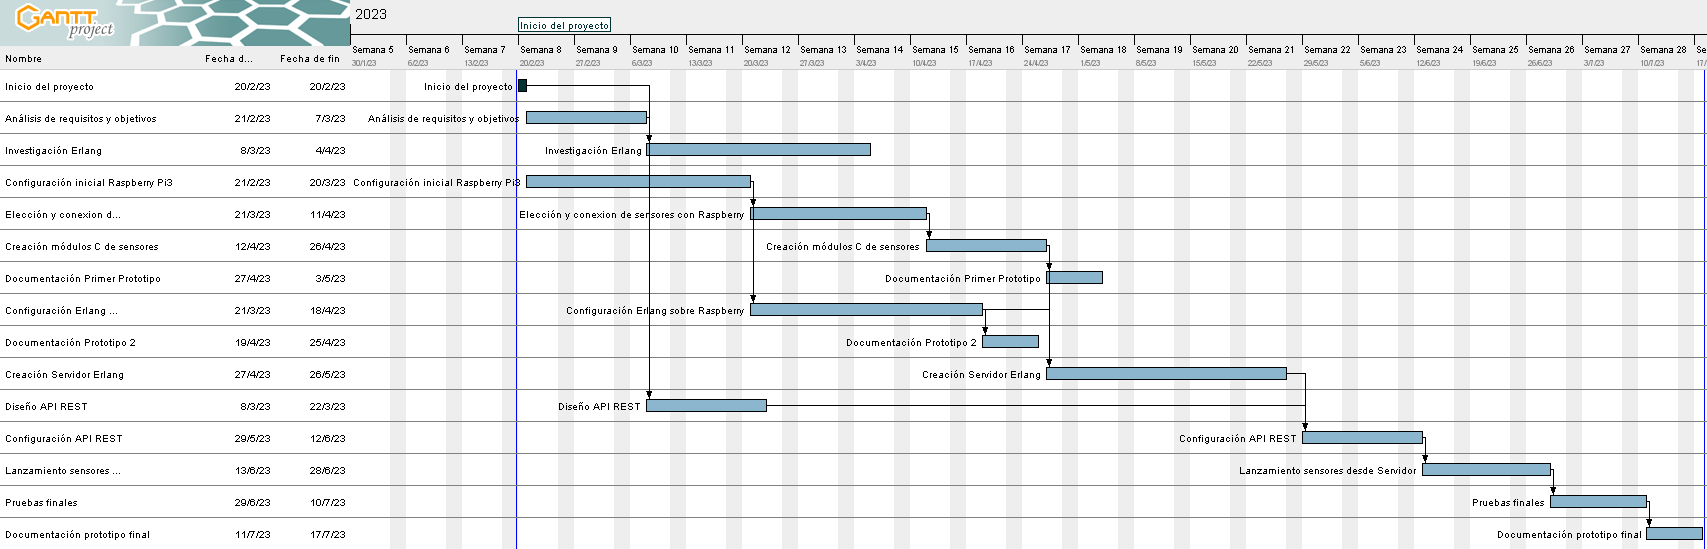
\includegraphics[height=0.32\textheight,angle=90]{images/TFGGantt.png}
\caption[Diagrama de Gantt]{Diagrama Gantt de la planificación del proyecto}%
\label{fig:gantt}
\end{figure}

\clearpage
\section{Recursos a emplear}

Tras la definición de actividades se deben analizar los recursos necesarios para el desarrollo del poryecto, estos se pueden diferenciar en tres tipos: Humanos, materiales y tecnológicos.

\subsection{Recursos humanos}%
\label{sec:recHumanos}

Estos recursos se miden contando las horas de trabajo de los desarrolladores, por ello, utilizando las actividades definidas y el tiempo disponible, se realiza una estimación del esfuerzo en horas de trabajo para desarrollarlas. Se estima la realización del proyecto en un periodo de 4 meses y 300 horas totales para la realización de los tres prototipos. Es por ello que se disponen de 88 días hábiles por lo que se deberán emplear una media de 3.4 horas diarias para la la finalización a tiempo del proyecto. 
El coste de estas horas se ha obtenido a través de la referencia bibliográfica \cite{Cowork2023}.

En la Tabla~\ref{tab:costSoft} puede observarse la estimación de horas necesarias para la realización de las diferentes actividades principales del proyecto.

\begin{table}[h]
\begin{center}
\begin{tabular}{|l|c|}
\hline
\rowcolor{gray!20}
\textbf{Software} & \textbf{Cantidad (Horas)} \\
\hline
Configuración de Raspberry-Pi & 30 \\
\hline
Conexión de sensores & 30\\
\hline
Programación de sensores & 55\\
\hline
Pruebas de frecuencia & 40 \\
\hline
Programación Servidor Erlang & 70\\
\hline
Pruebas de uso y cumplimiento requisitos & 30 \\
\hline
Documentación & 45 \\
\hline
\rowcolor{gray!20}
\textbf{Total} & \textbf{300}\\
\hline
\end{tabular}
\caption[Estimación de horas de trabajo]{Estimación de la distribución de horas de trabajo por actividades.}%
\label{tab:costSoft}
\end{center}
\end{table}

\subsection{Recursos materiales}%
\label{sec:recHardware}

En cuanto a los recursos materiales para el desarrollo del proyecto se requiere de:

\begin{itemize}
    \item Laboratorio (coworking).
    \item Ordenador (renting).
    \item Monitor (renting).
    \item Hardware (Adquirido).
    \item Licencias Software (Adquirido).
\end{itemize}

El hardware estimado que debe adquirirse es el mostrado en la Tabla~\ref{tab:recHard}.
\begin{table}[h]
\begin{center}
\sffamily
\begin{tabular}{|l|c|r|}
\hline
\rowcolor{gray!20}
\textbf{Componente} & \textbf{Cantidad}  & \textbf{Precio}  \\
\hline
Kit Raspberry-Pi 3 & 1 & 80\officialeuro  \\
\hline
Sensores & 5 & 35\officialeuro \\
\hline
Jumper Wire Cables & 3x40 pcs & 8\officialeuro \\
\hline
Resistencias 2.2K\(\Omega\) & 10 pcs & 2\officialeuro \\
\hline
Resistencias 1K\(\Omega\) & 10 pcs & 2\officialeuro \\
\hline
\rowcolor{gray!20}
\textbf{Total} & & \textbf{127\officialeuro} \\
\hline
\end{tabular}
\caption[Costes de componentes hardware]{Costes estimados de Hardware necesarios para la realización del proyecto}%
\label{tab:recHard}
\end{center}
\end{table}

\subsection{Recursos tecnológicos}

Para el desarrollo del proyecto se requiere del siguiente software de pago, en esta sección no aparece todo aquel software gratuito utilizado:

\begin{itemize}
    \item Licencia de Windows 10 Profesional.
    \item Licencia Office.
\end{itemize}

\subsection{Costes estimados del proyecto}

Por último, se presentan los costes del proyecto sumando todos los tipos de recursos requeridos, el sueldo por hora para los recursos humanos (trabajo) se ha obtenido mediante la Web Talent \cite{Cowork2023}. Para ello se ha escogido la media de los sueldos de los puestos especializados en cada fase, el resultado obtenido ha sido 19\officialeuro/hora.

En la Tabla~\ref{tab:costesTot} puede observarse el conjunto de todos los recursos junto con la cantidad necesaria de tiempo y su coste. Se ha obtenido una estimación total del proyecto de 7122\officialeuro.


\begin{table}[h]
\begin{center}
\sffamily
\begin{tabular}{|l|c|c|r|}
\hline
\rowcolor{gray!20}
\textbf{Recurso} & \textbf{Cantidad} & \textbf{Unidad} & \textbf{\officialeuro Total}  \\
\hline
Recurso Humano &  300 horas & 19\officialeuro/hora  \cite{Cowork2023}& 6000 \\
\hline
Laboratorio Coworking &  4 meses & 125\officialeuro/mes & 365  \\
\hline
Ordenador Renting &  4 meses & 125\officialeuro/mes & 200  \\
\hline
Monitor renting &  4 meses & 25\officialeuro/mes & 100  \\
\hline
Licencia Windows 10&  1 &  260\officialeuro & 260  \\
\hline
Licencia Office &  1 &  70\officialeuro & 70  \\
\hline
Recursos Hardware &  Tabla~\ref{tab:recHard} & 127\officialeuro & 127  \\
\hline
\rowcolor{gray!20}
\textbf{Total} & & & \textbf{7122\officialeuro} \\
\hline
\end{tabular}
\caption{Costes totales estimados del proyecto}%
\label{tab:costesTot}
\end{center}
\end{table}







